\section{Traffic Simulation Software}

The basis for the implementation will be set by a traffic simulation software. The requirements for this software were defined in \ref{trafficSimulationRequirements}. Based on an internet research the three traffic simulators CityTrafficSimulator, MATSim and CORSIM were preselected and will now be compared with the ten requirements.

...CityTrafficSimulator...

The second option for the traffic simulation is MATSim, an open source traffic simulation written in Java. It has built in support for car traffic simulation, but not for pedestrian traffic. However it is possible to extend MATSim with different locomotion types. There is for example a project that simulated airplane traffic over europe with MATSim.

MATSim on its own does not have a graphical display. It only puts out log files of what happened in the process of the simulation. However there is an extension that displays in real time what is happening in the simulation. It is called OTFVis. This extension as it is open source too can be expanded by the user.

\begin{figure}[!ht]
  \centering
  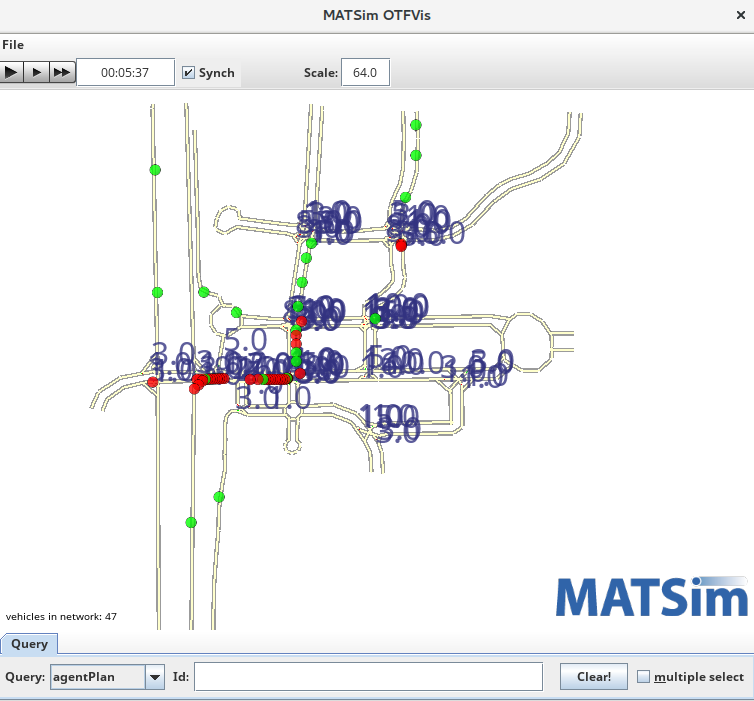
\includegraphics[width=12cm]{figures/otfvis}
  \caption[Screenshot of OTFVis]{Screenshot of OTFVis \protect\footnotemark}
  \label{otfvis}
\end{figure}

\footnotetext{screenshot}

Figure \ref{otfvis} shows the extension OTFVis for MATSim with debugging output patched in. It uses OpenGL to render to the screen and is relatively easy to extend with text output.

MATSim has different events and data structures that allow to interface with the simulation and read and write data from and to the simulation. The open source nature of MATSim also allows to expose all information wanted by compiling a custom version of MATSim.

MATSim has no built in traffic sensors or traffic lights, but like for the visual output, for traffic lights there is an extension that also allows for the dynamic control of the traffic lights.

...CORSIM...

%http://www.cszb.net/
%https://github.com/Schulteatq/CityTrafficSimulator/tree/master/CityTrafficSimulator

\begin{table}[!ht]
  	\centering
  	\begin{tabular}{l|l|l|l}
		 & CityTrafficSimulator & MATSim & CORSIM \\[10pt]
		Requirement & & & \\[10pt]
		R1 & yes & yes & yes \\[10pt]
		R2 & no & possible & no \\[10pt]
		R3 & yes & possible & yes \\[10pt]
		R4 & possible & possible & no \\[10pt]
		R5 & possible & yes & yes \\[10pt]
		R6 & no & no & no \\[10pt]
		R7 & yes & possible & yes \\[10pt]
		R8 & possible & possible & possible \\[10pt]
		R9 & yes & possible & yes \\[10pt]
		R10 & no & no & no \\[10pt]
		Other & & & \\[10pt]
		Open Source & yes & yes & no \\[10pt]
		Prog. Language & C\# & Java & C++, FORTRAN, ... \\[10pt]
	\end{tabular}
  	\caption{Traffic Simulation Software Requirements}
  	\label{simulationRequirementsComparison}
\end{table}

Table \ref{simulationRequirementsComparison} summarizes the result of the traffic simulator comparison. The value ``possible'' means that it is not included in the main program, but can be done through some external program or extension.

MATSim was chosen as the simulation for the traffic light control system. As can be seen in table \ref{simulationRequirementsComparison}, all three traffic simulations have almost the same feature set regarding the requirements, but in comparison to CORSIM, MATSim was chosen, because it is open source and with a project that might have to expand on the simulation it uses, open source fits really well to the traffic signal control system. In comparison to CityTrafficSimulator, MATSim with the extensions OTFVis and Signals, both fulfilled the same requirements, but the community surrounding MATSim, the other extensions and the whole feature set is more complete.

\subsection*{Dependency Injection}

TODO complete this

\section{Scenario generation}
\label{scenario_generation}

TODO complete this

\section{Neural Network Library}

\section{Prediction Network Implementation}

We tried the prediction network with an input for the amount of cars that want to pass, but this did introduce unnecessary complexity and the accuracy of the network went down

learning rule

artificial neural network type
